\section{Background and Objectives}\label{sec:bg}

\begin{table*}[]
\centering
\begin{tabular}{|l|l|l|l|l|}
\hline
 & \textbf{Trigger-based} & \textbf{Driver functions} & \textbf{Orchestrator} & \textbf{unum} \\ \hline
\textit{Purely Serverless}          & \cmark & \cmark & \xmark & \cmark \\ \hline
\textit{Higher-level interface}     & \xmark & \xmark & \cmark & \cmark \\ \hline
\textit{Exactly-once semantics} & \xmark & \xmark & \cmark & \cmark \\ \hline
\textit{Avoid double billing}       & \cmark & \xmark & \cmark & \cmark \\ \hline
\end{tabular}
\caption{Comparison with existing approaches}
\label{table:positioning}
\end{table*}


% Large-scale applications composed of many functions~\cite{excamera, gg-atc,
% deathstar} introduce several new challenges to serverless computing. 

In this section, we describe why it is hard to compose large serverless
workflows, why a purely serverless architecture is interesting and what our
objectives are.

\subsection{Evolution of Serverless Workflows}

\begin{figure}[t!]
    \centering
    \scalebox{.7}{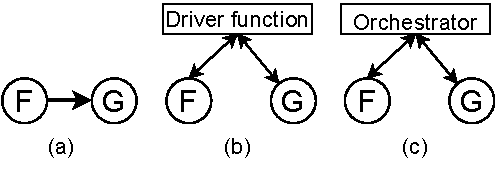
\includegraphics[width=\columnwidth]{figures/ChainExample.pdf}}
    \caption{Chaining two functions with triggers, driver functions and
    orchestrators. In the trigger-based approach, \texttt{F} asynchronously
    invokes \texttt{G} with \texttt{F}'s result. In the driver functions
    approach, a driver function first synchronously invokes \texttt{F},
    usually via HTTP, and after \texttt{F} returns, synchronously invokes
    \texttt{G} with \texttt{F}'s result. Workflow orchestrators is
    architecturally similar to driver functions. An orchestrator instance
    invokes \texttt{F}, waits for \texttt{F} to return and then invokes
    \texttt{G} with \texttt{F}'s result.}
    \label{fig:chain-example}
\end{figure}

\subsubsection{Ad-hoc composition: triggers and driver functions}

The original serverless abstraction is designed around individual functions
and does not provide an interface for programming larger applications with
many functions. As a result, early adopters use low-level function invocation
APIs to compose functions in an ad-hoc manner, and there are two primary
approaches.

The first approach is called trigger-based or unstructure
composition~\cite{netherite} where functions invoke each other
\emph{asynchronously} via storage triggers. The second is called driver
functions~\cite{beldi} where a single function invokes other functions
\emph{synchronously}. Figure~\ref{fig:chain-example} depicts an example of
chaining functions with the two approaches.

Although both approaches are purely serverless and do not require adding
additional components to the serverless infrastructure, they each has
important drawbacks. Unstructured composition scatters control flow across
constituent functions. As the number of functions increases, development can
quickly get unwieldy. Moreover, it does not support important composition
patterns such as fan-in, where we want to invoke a function to aggregate the
results of multiple upstream functions only after all of them are complete.

\dhl{Maybe explain why fan-in is not supported as a contrast to \name{}. But
tricky because there's nothing fundamentally stopping unstructured composition
from achieving fan-in as \name{} also demonstrated. Maybe the main difference
is ad-hoc vs ..not. Or maybe the main difference is the addition of strongly
consistent data stores and how we use them.}

Compared with unstructured composition, driver functions concentrate control
flow in a single function and supports aggregation. However, users pay for the
time when driver functions idly wait for callees to return. This causes
\emph{double billing}~\cite{double-billing}. Also, serverless platforms
commonly impose timeouts. A driver function instance has to wait until all
functions in the application are complete, which risks timeouts and limits
application scale.

Moreover, both approaches suffer from weak execution guarantees of the
underlying serverless system. Functions can crash mid-execution due to runtime
or hardware faults which may lead to automatic retries~\cite{aws-lambda-retry,
azure-functions-retry}. Even in the absence of faults, most serverless
platforms only ensure at-least-once execution~\cite{aws-lambda-async-invoke,
azure-functions-exec-guarantee} so a single invocation can trigger multiple,
potentially concurrent, instances.

\subsubsection{Workflow orchestrators}

Recently, workflow orchestrators have emerged to tackle the challenges of
large serverless applications~\cite{excamera, gg-atc, aws-step-functions,
google-cloud-composer, google-workflows, durable-functions}. Orchestrators are
separate hosted services that execute workflow definitions, invoke constituent
functions and manage workflow states. Architecturally, they are similar to
driver functions (Figure~\ref{fig:chain-example}). For every workflow
invocation, an orchestrator instance invokes a constituent function, waits for
its result and passes it to downstream functions via invocation. All functions
invocation are initiated by the orchestrator and all states (e.g., function
results) pass through the orchestrator.

Different from ad-hoc composition, orchestrators offer (1). higher-level
programming interfaces that directly express function interactions and hide
low-level APIs, (2). a rich set of composition primitives, including
branching, chaining, fan-out and fan-in, (3). exactly-once semantics for
workflow execution, and (4). long or no runtime limits.

While fixing the flaws of ad-hoc composition, the orchestrator design creates
several important drawbacks that neglect or even compromise key benefits of
the serverless abstraction: (1). End-to-end performance now also depends on
the orchestrator service that is separate from the FaaS engine. A slow
orchestrator can become a bottleneck and nullify the fast autoscale advantage
of serverless. (2). Serverless computing already offers compute and storage
building blocks that are highly performant and scalable. Adding yet another
separate service that is a mixture of compute and storage is repeating the
difficult and expensive task of developing and maintaining a large-scale system,
which often requires a dedicated engineering team.(3). Platform-specific
orchestrators force developers to write with proprietary APIs and locks them
in a particular cloud provider.\dhl{I'm hesitant to include the 3rd point
because 1. we can't demonstrate that \name{} solves this problem. 2. while
it's a benefit, it feels more an engineering problem than a research problem.
3. FaaS functions are already platform-specific. Lambda, Azure functions, etc.
all have different propritary APIs.}

\subsection{Research question and objectives}

In this paper, we examine whether we can have the best of both worlds. We
argue that it is possible to preserve the advantages of workflow orchestrators
while building entirely on top of the existing serverless computing
abstraction without adding any supplemental components.

Specifically, we aim for a system with the following objectives:

\paragraph{\emph{Purely serverless}} The system should work within the current
serverless environment and not require adding any new services.

The system should execute workflows solely as event-driven serverless
functions, and use serverless storage, when necessary, to enable stateful
operations (e.g., fan-in).

\paragraph{Higher-level programming interface} Developers should express
function compositions with higher-level primitives similar to exising workflow
orchestrators (e.g., AWS Step Functions) instead of ad-hoc mechanisms.

\paragraph{Supports all common interactions} The system should support all
composition patterns commonly used in orchestrators today, including chaining,
branching, fan-out and fan-in.

\paragraph{Exactly-once semantics} Even if a function executes multiple times,
due to retries or duplicate invocations, concurrently or non-concurrently, the
final state should appear that the execution happened only once.

\paragraph{Avoids double billing} Users should only pay for the resources
used. Functions should not synchronously wait for other functions to return.

\paragraph{Comparable performance and costs} The system should at least have
comparable costs and performance as the state-of-the-art workflow
orchestrators.
